\chapter{Adaptações das plantas e plasticidade fenotípica}\label{ch:b2:plant-plasticity}

Duas folhas do mesmo carvalho: a do topo da copa é pequena, espessa e
coriácea; a do interior sombreado, três vezes maior e fina como papel.
Uma plântula do mesmo carvalho sob um dossel fechado cresce alta e
franzina; sua irmã numa clareira fica baixa e robusta. Nenhuma das duas
diferenças é genética. Uma planta não pode caminhar até um lugar
melhor, por isso se constrói para se ajustar ao lugar que tem: percebe
a luz, a gravidade, o toque, a água, o sal, o frio, e se curva,
engrossa, se alonga, fecha seus poros ou endurece suas células de
acordo com isso. Este capítulo trata dessa plasticidade --- como uma
planta lê o ambiente e o que ela faz a respeito --- e das \omterm{def:b2:plant-plasticity:plasticity}{adaptações}
hereditárias pelas quais as linhagens se ajustaram aos desertos, à
sombra, ao sal e à geada.

\section{A plasticidade e seus limites}

\begin{definition}[Plasticidade fenotípica e norma de reação]\label{def:b2:plant-plasticity:plasticity}
\index{plasticidade fenotípica}\index{norma de reação}\index{aclimatação}\index{adaptação}
A \emph{plasticidade fenotípica} é a capacidade de um \omterm{def:b2:meiosis-heredity:vocabulary}{genótipo} de
produzir \omterm{def:b2:meiosis-heredity:vocabulary}{fenótipos} diferentes em ambientes diferentes. A \emph{norma de
reação} de um \omterm{def:b2:meiosis-heredity:vocabulary}{genótipo} é a curva de seu \omterm{def:b2:meiosis-heredity:vocabulary}{fenótipo} em função de uma
variável ambiental --- a espessura da folha em função da luz, o
comprimento do caule em função da temperatura; os \omterm{def:b2:meiosis-heredity:vocabulary}{genótipos} diferem em
suas normas, e as diferenças são hereditárias mesmo quando a própria
plasticidade não o é. A \emph{aclimatação} é a forma reversível,
fisiológica: uma folha que espessa a cutícula numa semana seca, uma
célula que produz anticongelante no outono. A \emph{adaptação}, no
sentido evolutivo, é o ajuste hereditário de uma linhagem a seu
hábitat, selecionado ao longo das gerações; um cacto está adaptado à
seca, um feijoeiro se aclimata a um período seco. As plantas são mais
plásticas que os animais porque são modulares e de crescimento
indeterminado (\cref{ch:b2:plant-meristems}): a próxima folha pode ser construída de modo
diferente da anterior, e a vida séssil faz da plasticidade a única
maneira de se mover.
\end{definition}

\begin{omfigure}
\begin{tikzpicture}
\begin{axis}[
  width=0.72\linewidth, height=5.4cm,
  axis x line=bottom, axis y line=left,
  xmin=0, xmax=100, ymin=0, ymax=1.2,
  xlabel={luz (\% do sol pleno)}, ylabel={espessura da folha (relativa)},
  xlabel style={font=\small, at={(axis description cs:0.5,-0.13)}, anchor=north},
  ylabel style={font=\small},
  tick label style={font=\small}, xtick={0,25,50,75,100}, ytick={0,0.5,1},
  legend style={font=\scriptsize, at={(0.97,0.08)}, anchor=south east, draw=none},
  clip=false,
]
\addplot[very thick, omDef, domain=2:100, samples=60] {0.35 + 0.65*(1-exp(-x/30))};
\addlegendentry{genótipo 1: um carvalho plástico}
\addplot[very thick, omThm, domain=2:100, samples=60] {0.55 + 0.2*(1-exp(-x/30))};
\addlegendentry{genótipo 2: um menos plástico}
\end{axis}
\end{tikzpicture}

{\small Duas \omterm{def:b2:plant-plasticity:plasticity}{normas de reação}. Cada \omterm{def:b2:meiosis-heredity:vocabulary}{genótipo} forma folhas mais espessas
com mais luz; a inclinação da curva --- a plasticidade --- é ela mesma
um caráter hereditário, e os dois \omterm{def:b2:meiosis-heredity:vocabulary}{genótipos} diferem nele.}
\end{omfigure}

\begin{proposition}[Folhas de sol e folhas de sombra]\label{prop:b2:plant-plasticity:sunshade}
\index{folha de sol}\index{folha de sombra}
Uma folha que se desenvolve em sol pleno é pequena, espessa, com duas
ou três camadas de células paliçádicas, muitos estômatos, uma cutícula
espessa, uma alta concentração da enzima que fixa o carbono e uma alta
taxa máxima de fotossíntese; uma folha da mesma planta que se
desenvolve na sombra é grande, fina, com uma camada paliçádica, mais
clorofila por unidade de massa, uma baixa taxa de respiração e um
baixo ponto de compensação luminoso. A \omterm{prop:b2:plant-plasticity:sunshade}{folha de sombra} é construída
para captar cada fóton a um custo mínimo; a \omterm{prop:b2:plant-plasticity:sunshade}{folha de sol}, para usar uma
enxurrada deles sem superaquecer nem murchar. A decisão é tomada
enquanto a folha ainda é um primórdio, a partir da luz --- e em
particular de sua cor --- que chega à gema; uma folha madura não
consegue se reconstruir, e é por isso que uma planta levada da sombra
para o sol se queima até formar folhas novas.
\end{proposition}

\begin{omfigure}
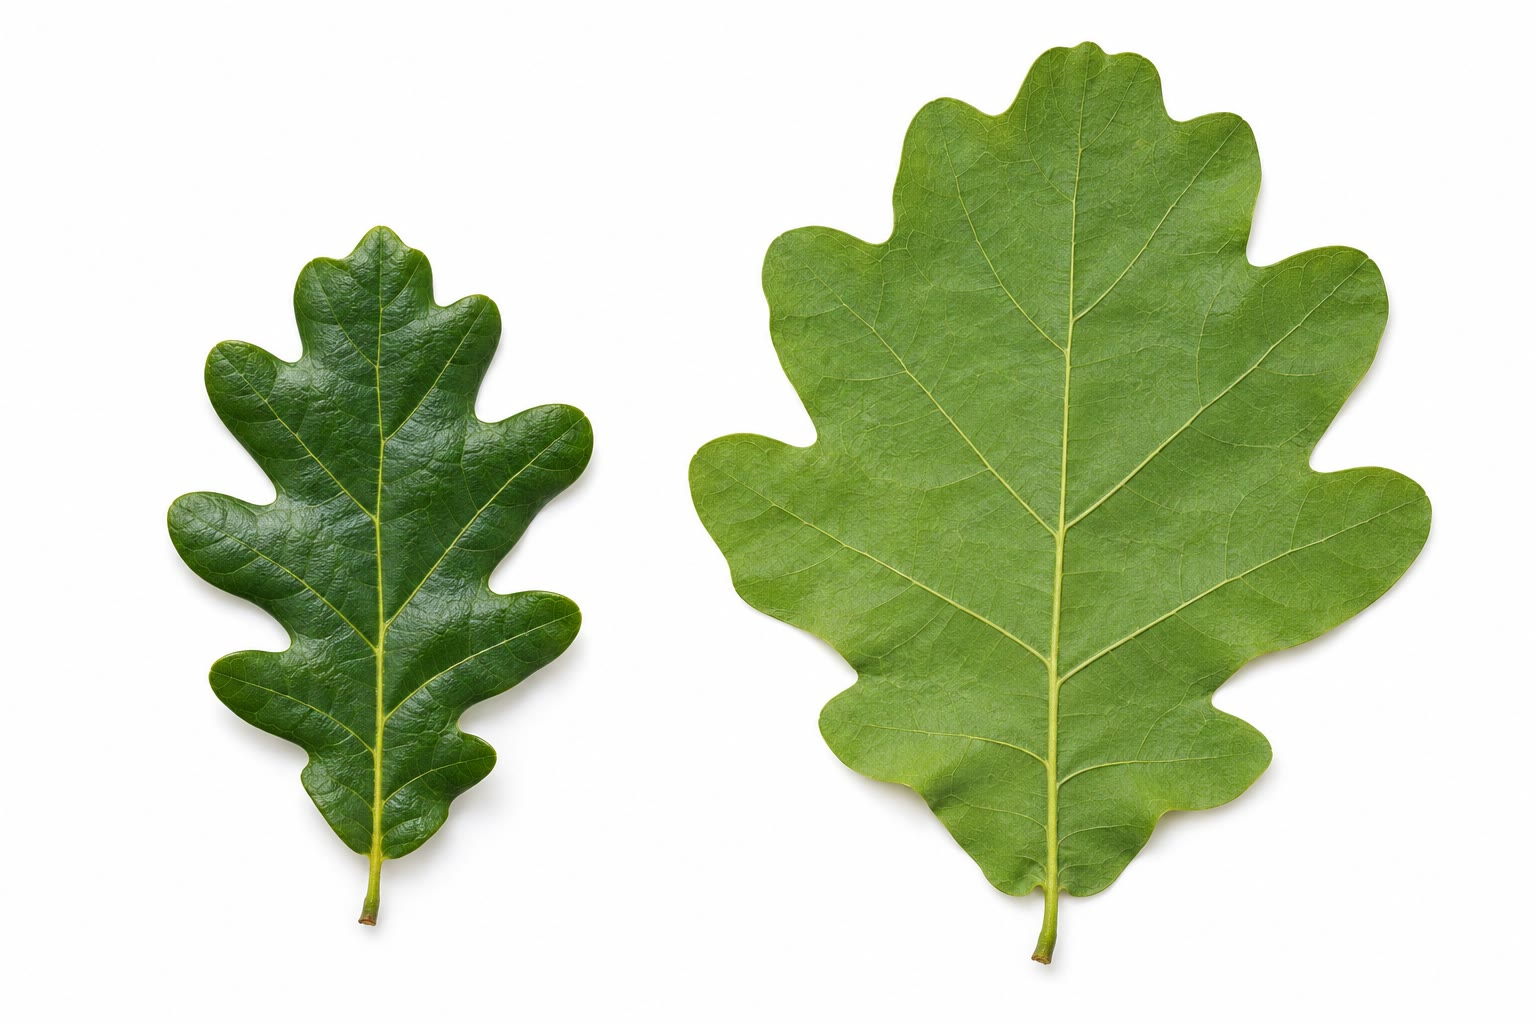
\includegraphics[width=0.55\linewidth]{images/book4/ai/b4-15-sun-shade-leaves.jpg}

{\small Uma \omterm{prop:b2:plant-plasticity:sunshade}{folha de sol} e uma \omterm{prop:b2:plant-plasticity:sunshade}{folha de sombra} de um mesmo carvalho:
mesmo \omterm{def:b2:meiosis-heredity:vocabulary}{genótipo}, luz diferente, folhas diferentes.}
\end{omfigure}

\section{A leitura da luz}

\begin{theorem}[O fitocromo como medidor da qualidade da luz]\label{thm:b2:plant-plasticity:phytochrome}
\index{fitocromo}\index{razão vermelho:vermelho extremo}\index{evitação da sombra}
O fitocromo existe em duas formas: $P_r$, que absorve a luz vermelha
(\qty{660}{nm}) e é convertida em $P_{fr}$, e $P_{fr}$, que absorve o
vermelho extremo (\qty{730}{nm}) e é convertida de volta --- e é
$P_{fr}$ que age. Sob luz contínua, as duas conversões se equilibram
num \emph{fotoequilíbrio} cuja posição depende apenas da razão entre
vermelho e vermelho extremo na luz:
\[
\varphi = \frac{P_{fr}}{P_{r} + P_{fr}} = \frac{R}{R + a\,FR},
\]
em que $R$ e $FR$ são as densidades de fluxo de fótons nas duas faixas
e $a$ é uma constante do pigmento ($a \approx 0.77$). A luz do sol tem
$R{:}FR \approx 1.15$, o que dá $\varphi \approx 0.6$; a luz filtrada
pelas folhas, que absorvem o vermelho e transmitem o vermelho extremo,
tem $R{:}FR
\approx 0.2$ e $\varphi \approx 0.2$. Um $\varphi$ baixo informa a uma
planta que ela está sob outras plantas ou ao lado delas antes mesmo de
estar de fato sombreada --- o vermelho extremo refletido por uma
vizinha é detectado no lado voltado para ela --- e ela responde com a
\emph{síndrome de \omterm{thm:b2:plant-plasticity:phytochrome}{evitação da sombra}}: alongamento mais rápido do
caule, pecíolos mais longos, folhas erguidas, menos ramificação,
floração mais precoce. Uma plântula sob um dossel fechado dobra sua
taxa de alongamento.
\end{theorem}
\begin{proof}
Seja $k_1 R$ a constante de velocidade de $P_r \to P_{fr}$
(proporcional ao fluxo de vermelho) e $k_2\,FR$ a de $P_{fr} \to P_r$.
No equilíbrio, $k_1 R\,P_r = k_2\,FR\,P_{fr}$, de modo que
$P_{fr}/P_r = k_1 R/
(k_2 FR)$ e $\varphi = P_{fr}/(P_r + P_{fr}) = R/(R + a\,FR)$, com
$a = k_2/k_1$. (As duas formas absorvem um pouco nas duas faixas, o que
a constante $a$ incorpora; a forma do resultado não muda.) Com
$a = 0.77$: $1.15/(1.15 + 0.77) = 0.60$; $0.2/(0.2 + 0.77) = 0.21$.
\end{proof}

\begin{omfigure}
\begin{tikzpicture}
\begin{axis}[
  width=0.7\linewidth, height=5.2cm,
  axis x line=bottom, axis y line=left,
  xmin=0, xmax=1.4, ymin=0, ymax=0.8,
  xlabel={razão vermelho : vermelho extremo da luz}, ylabel={$\varphi = P_{fr}/P_{\text{total}}$},
  xlabel style={font=\small, at={(axis description cs:0.5,-0.13)}, anchor=north},
  ylabel style={font=\small},
  tick label style={font=\small}, xtick={0,0.2,0.6,1.15}, ytick={0,0.2,0.4,0.6},
  clip=false,
]
\addplot[very thick, omDef, domain=0:1.4, samples=60] {x/(x+0.77)};
\draw[dashed, gray] (axis cs:1.15,0) -- (axis cs:1.15,0.6) -- (axis cs:0,0.6); \node[font=\scriptsize, anchor=south west] at (axis cs:1.15,0.6) {sol aberto};
\draw[dashed, gray] (axis cs:0.2,0) -- (axis cs:0.2,0.21) -- (axis cs:0,0.21); \node[font=\scriptsize, anchor=west] at (axis cs:0.25,0.15) {sob um dossel};
\end{axis}
\end{tikzpicture}

{\small O fotoequilíbrio do fitocromo em função da razão vermelho /
vermelho extremo. A luz do sol mantém a maior parte do pigmento na
forma ativa; a luz filtrada pelas folhas o mantém sobretudo inativo, e
a planta interpreta a diferença como a presença de vizinhas.}
\end{omfigure}

\begin{proposition}[Fototropismo]\label{prop:b2:plant-plasticity:phototropism}
\index{fototropismo}\index{tropismo}\index{hipótese de Cholodny--Went}
Um \emph{tropismo} é um movimento de crescimento orientado por um
estímulo direcional. No \emph{fototropismo}, um caule se curva em
direção à luz azul: a luz é percebida na ponta por um receptor de luz
azul (a fototropina), a auxina que desce da ponta é redirecionada para
o lado sombreado --- seus transportadores se deslocam para a membrana
lateral --- e o lado sombreado, recebendo mais auxina, se alonga mais
depressa que o lado iluminado, de modo que o caule se curva em direção
à luz. A curvatura é crescimento diferencial, e não um músculo: ela só
ocorre na \omterm{prop:b2:plant-meristems:ram}{zona de alongamento}, leva uma ou duas horas e é
irreversível. As raízes, nas quais o mesmo excesso de auxina
\emph{inibe} o alongamento, se curvam para o lado oposto.
\end{proposition}
\begin{proof}[Evidências]
Darwin (1880) mostrou com coleóptilos de gramíneas que a ponta percebe
a luz e que a zona abaixo dela se curva: cobrir a ponta com um capuz
opaco abolia a curvatura, cobrir a base com um tubo não, e um capuz
transparente a deixava intacta. Boysen-Jensen (1913) cortou a ponta e a
recolocou com um bloco de gelatina entre as partes: a curvatura
persistia, de modo que o sinal era uma substância difusível; uma lâmina
de mica inserida no lado sombreado a bloqueava, e no lado iluminado
não, de modo que a substância descia pelo lado sombreado. Went (1928)
coletou a substância em ágar a partir de pontas cortadas e verificou
que um bloco colocado fora do centro sobre um coleóptilo decapitado, no
escuro, o fazia curvar-se para o lado oposto ao bloco --- num ângulo
proporcional à quantidade --- e, coletando ágar das duas metades de uma
ponta iluminada de um só lado, encontrou cerca de dois terços da
auxina no lado sombreado e um terço no lado iluminado (Briggs, 1957,
com métodos melhores). A redistribuição lateral de um hormônio de
crescimento é a \omterm{prop:b2:plant-plasticity:phototropism}{hipótese de Cholodny--Went}, e ela se manteve.
\end{proof}

\begin{omfigure}
\begin{tikzpicture}[every node/.style={font=\scriptsize}, >=stealth]
  \foreach \x/\lab/\cap/\bend in {0/{intacto:\\curva-se}/0/1, 2.6/{ponta coberta:\\sem curvatura}/1/0, 5.2/{base coberta:\\curva-se}/2/1, 7.8/{ponta cortada:\\sem curvatura}/3/0, 10.4/{ponta sobre gelatina:\\curva-se}/4/1} {
    \begin{scope}[xshift=\x cm]
      \fill[omExo!30] (-0.7,0) rectangle (0.7,0.2);
      \ifnum\bend=1
        \draw[very thick, omExo!70!black] (0,0.2) -- (0,1.6) .. controls (0,2.3) and (0.5,2.6) .. (0.9,2.8);
      \else
        \draw[very thick, omExo!70!black] (0,0.2) -- (0,3.0);
      \fi
      \ifnum\cap=1 \fill[black] (-0.2,2.7) rectangle (0.2,3.1); \fi
      \ifnum\cap=2 \fill[black] (-0.2,0.2) rectangle (0.2,1.5); \fi
      \ifnum\cap=3 \draw[thick] (-0.3,2.6) -- (0.3,2.6); \fi
      \ifnum\cap=4 \fill[omDef!35] (-0.2,2.55) rectangle (0.2,2.75); \draw[very thick, omExo!70!black] (0.55,2.75) -- (0.9,3.1); \fi
      \node[below, align=center] at (0,-0.15) {\lab};
    \end{scope}
  }
  \node[anchor=east, align=right, omProp!80!black] at (-1.0,2.2) {luz vinda da\\direita $\to$};
\end{tikzpicture}

{\small Os experimentos com coleóptilos. Darwin: a ponta percebe a luz
e a região abaixo dela se curva; cobrir a ponta impede a curvatura,
proteger a base não. Boysen-Jensen: o sinal atravessa um bloco de
gelatina --- é uma substância.}
\end{omfigure}

\begin{omfigure}
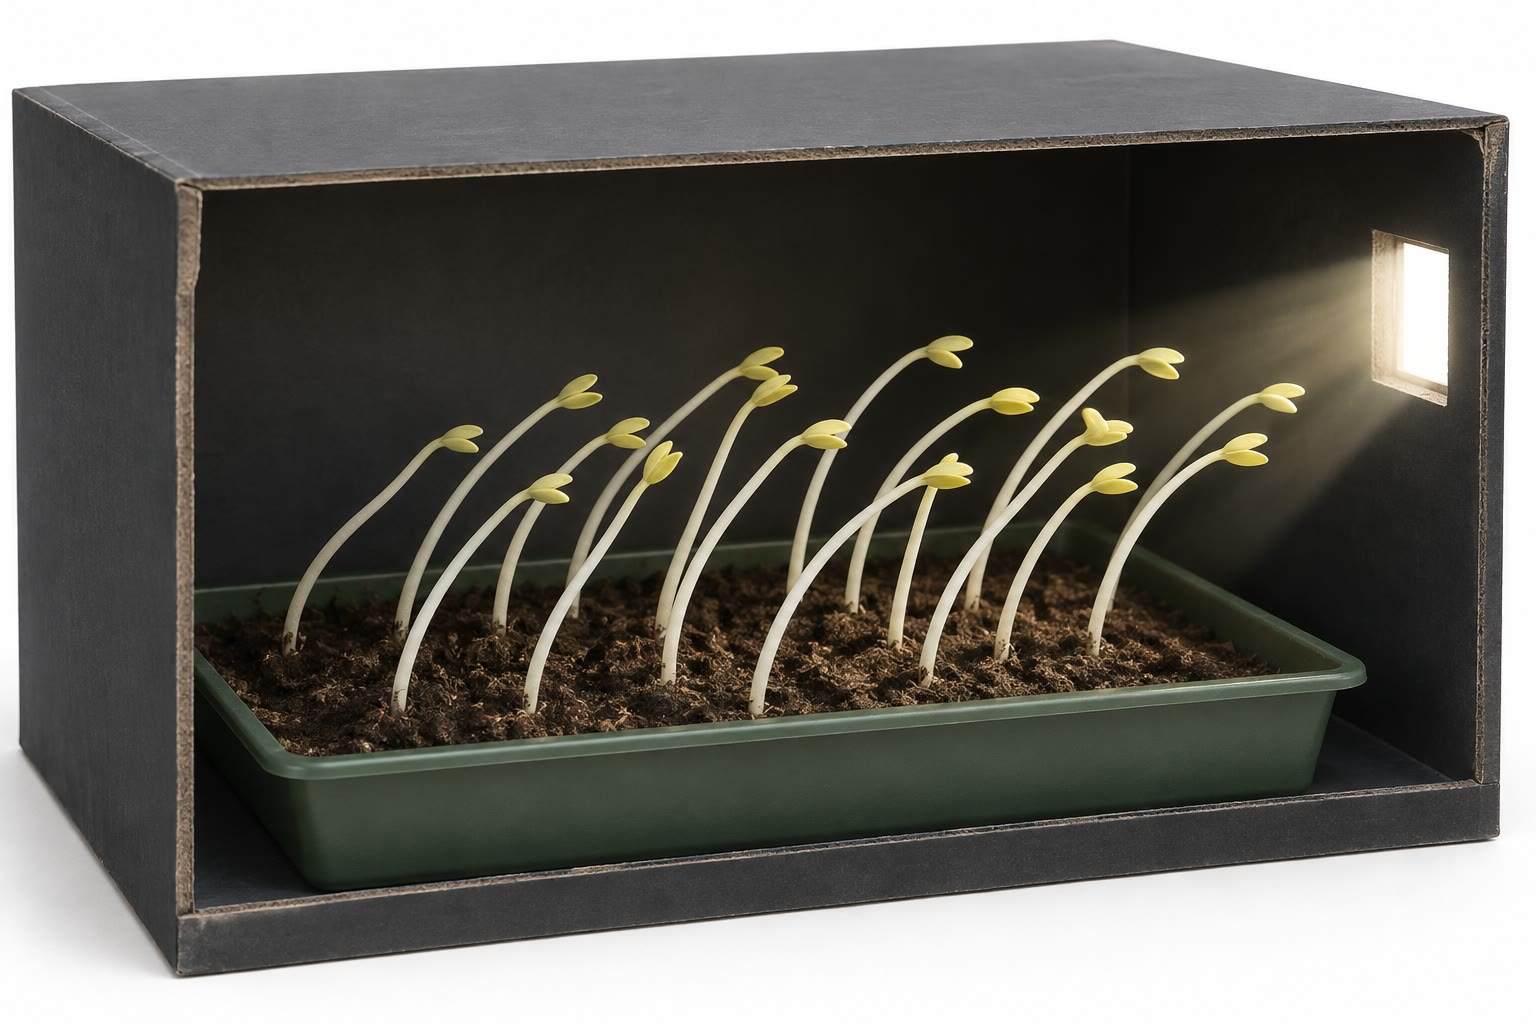
\includegraphics[width=0.55\linewidth]{images/book4/ai/b4-15-phototropism.jpg}

{\small Plântulas numa caixa com uma janela: todas se curvam em direção
à luz, crescendo mais depressa no lado oposto a ela.}
\end{omfigure}

\begin{theorem}[Quanto um caule se curva]\label{thm:b2:plant-plasticity:bend}
Se o lado sombreado de um caule de diâmetro $d$ se alonga de uma
quantidade relativa $\varepsilon_s$ e o lado iluminado de
$\varepsilon_l$ ao longo de uma zona de crescimento de comprimento $L$,
a zona se curva num ângulo
\[
\theta = \frac{L\,(\varepsilon_s - \varepsilon_l)}{d}
\]
(em radianos). Um coleóptilo que cresce \qty{5}{\%} por hora numa zona
de \qty{10}{mm} de comprimento e \qty{1}{mm} de diâmetro, com a auxina
repartida em
$65 : 35$, de modo que os dois lados crescem a $1.3$ e $0.7$ vezes a
média, se curva em três horas de $\theta = 10\times(0.195 - 0.105)/1 =
0.9$ radiano, cerca de \qty{50}{\degree}. A curvatura não exige nenhum
mecanismo novo: o crescimento comum do \cref{ch:b2:plant-meristems}, tornado desigual dos
dois lados, basta.
\end{theorem}
\begin{proof}
Os dois lados da zona se tornam arcos de raios $\rho + d/2$ e
$\rho - d/2$ que subtendem o mesmo ângulo $\theta$, de comprimentos
$L(1 +
\varepsilon_s)$ e $L(1 + \varepsilon_l)$; sua diferença é
$\theta d$, de modo que $\theta = L(\varepsilon_s - \varepsilon_l)/d$.
Em três horas a \qty{5}{\%} por hora, a extensão média é $0.15$;
$1.3\times 0.15 = 0.195$ e $0.7\times 0.15 = 0.105$.
\end{proof}

\begin{proposition}[Gravitropismo]\label{prop:b2:plant-plasticity:gravitropism}
\index{gravitropismo}\index{estatólito}
Um caule deitado de lado se volta para cima, e uma raiz para baixo, em
poucas horas. A direção da gravidade é percebida por
\emph{estatólitos} --- grãos de amido densos em células especializadas
da coifa e da bainha amilífera do caule ---, que sedimentam no lado
inferior da célula em segundos e, pressionando a membrana ou o retículo
endoplasmático, redirecionam os transportadores de auxina, de modo que
a auxina se acumula no lado inferior. No caule, o lado inferior cresce
mais depressa e o caule se curva para cima; na raiz, o mesmo excesso de
auxina inibe o lado inferior, o lado superior cresce mais depressa e a
raiz se curva para baixo. Retire a coifa e a raiz cresce reta em
qualquer direção; mutantes sem amido percebem mal a gravidade; uma raiz
sobre um tambor que gira lentamente (um clinostato), que nunca deixa os
estatólitos sedimentarem, cresce sem direção. A resposta é um segundo
uso do mecanismo de Cholodny--Went, com outro sensor.
\end{proposition}

\section{A água: fechar os poros}

\begin{proposition}[O controle estomático]\label{prop:b2:plant-plasticity:stomata}
\index{estômato}\index{célula-guarda}\index{ácido abscísico}\index{condutância estomática}
Os poros da folha, os \emph{estômatos}, são delimitados cada um por
duas \emph{células-guarda} cujas paredes são espessadas de modo
desigual, de modo que, quando absorvem potássio e água e incham, elas
se arqueiam e abrem o poro, e, quando os perdem, o fecham. Elas se
abrem pela manhã sob luz azul e baixo $\mathrm{CO_2}$ interno, e se
fecham no escuro; fecham-se em poucos minutos quando chega o
\emph{\omterm{def:b2:plant-flowering:dormancy}{ácido abscísico}} --- produzido nas raízes que percebem o solo
secando e levado para cima no xilema, ou produzido na própria folha
quando ela perde turgescência --- e quando o ar está muito seco. A
\emph{\omterm{prop:b2:plant-plasticity:stomata}{condutância estomática}} $g_s$ fixa ao mesmo tempo a água perdida,
$E = g_s\,(w_i - w_a)$ (a diferença de fração molar de vapor d'água
entre o interior da folha, saturado, e o ar), e o $\mathrm{CO_2}$
absorvido, $A = g_s\,(c_a -
c_i)/1.6$ (o fator $1.6$ sendo a razão entre as difusividades do vapor
d'água e do $\mathrm{CO_2}$). A folha troca água por carbono através de
uma única válvula, e sua \emph{eficiência do uso da água} é
\[
\frac{A}{E} = \frac{c_a - c_i}{1.6\,(w_i - w_a)},
\]
alguns milésimos de mol de carbono por mol de água: uma folha C$_3$
típica gasta \qtyrange{400}{600}{g} de água por grama de carbono
fixado; uma folha C$_4$, metade disso; uma \omterm{prop:b2:plant-plasticity:xerophytes}{planta CAM}, um quinto.
\end{proposition}

\begin{omfigure}
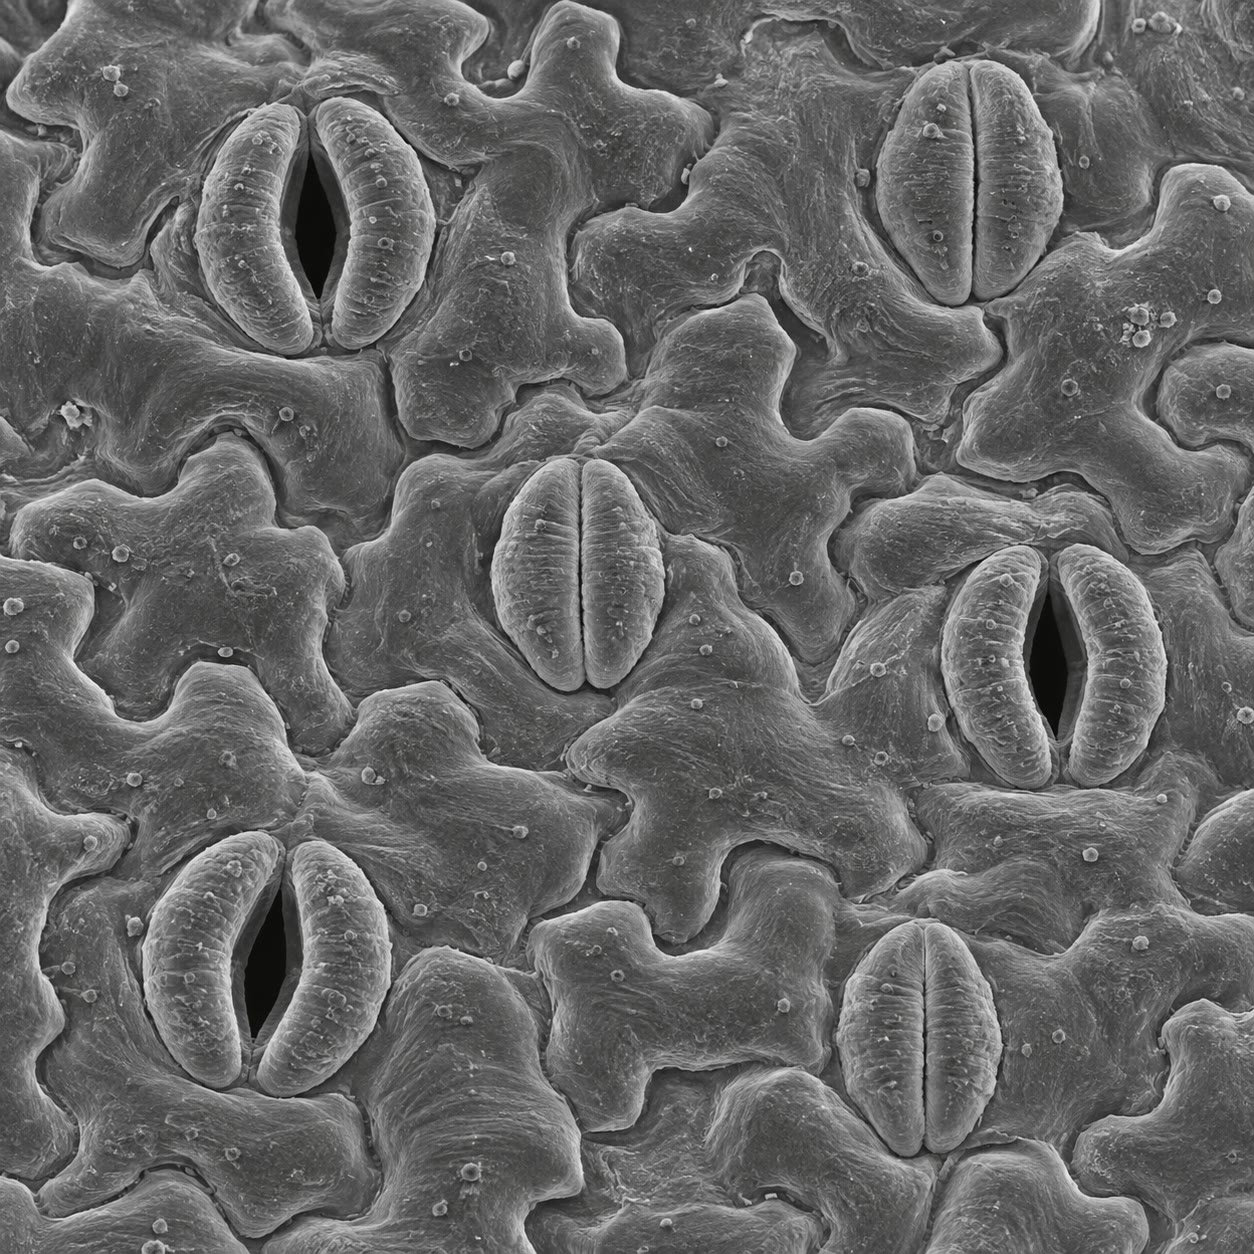
\includegraphics[width=0.42\linewidth]{images/book4/ai/b4-15-stomata-sem.jpg}

{\small Estômatos na face inferior de uma folha, alguns abertos e
outros fechados: duas células-guarda em torno de cada poro, a válvula
pela qual a folha troca água por dióxido de carbono.}
\end{omfigure}

\begin{example}[O custo do carbono de um dia]\label{ex:b2:plant-plasticity:wue}
Ao meio-dia, uma folha de girassol com
$g_s = \qty{0.3}{mol.m^{-2}.s^{-1}}$,
$w_i - w_a = 0.02$ e $c_a - c_i = \qty{120}{\micro mol/mol}$ transpira
$E = \qty{6}{mmol.m^{-2}.s^{-1}}$ e fixa $A =
0.3\times 120/1.6 = \qty{22}{\micro mol.m^{-2}.s^{-1}}$: $A/E =
\qty{3.7e-3}{}$, isto é, 270 moléculas de água para cada átomo de
carbono, \qty{400}{g} de água por grama de carbono. Um hectare dessas
folhas perde \qty{40}{t} de água num dia de verão para fixar
\qty{100}{kg} de carbono. Quando o solo seca, o \omterm{def:b2:plant-flowering:dormancy}{ácido abscísico} fecha
os estômatos a um décimo dessa condutância: $E$ cai dez vezes, $A$ menos
que isso (pois $c_i$ também cai), e a planta sobrevive com uma dieta de
fome, em vez de morrer de sede.
\end{example}

\begin{proposition}[Adaptações à seca]\label{prop:b2:plant-plasticity:xerophytes}
\index{xerófita}\index{planta CAM}\index{suculenta}
As plantas de lugares secos (\emph{xerófitas}) combinam estruturas e
estratégias hereditárias. Reduzir a perda: cutícula espessa, estômatos
afundados em criptas ou sob pelos (que espessam a camada de ar parado),
folhas reduzidas a espinhos (cacto) ou perdidas na estação seca, folhas
pequenas e espessas que se enrolam. Armazenar: caules e folhas
suculentos, com mucilagem que retém água. Alcançar: raízes de
\qty{50}{m} de profundidade (algaroba) ou espalhadas logo abaixo da
superfície para aproveitar uma pancada de chuva. Deslocar no tempo: as
\omterm{prop:b2:plant-plasticity:xerophytes}{plantas CAM} abrem os estômatos à noite, quando $w_i - w_a$ é pequeno,
fixam o $\mathrm{CO_2}$ em ácido málico e o refixam de dia, com os
estômatos fechados --- o mesmo carbono por um quinto da água. Escapar:
as anuais do deserto vivem como \omterm{def:b2:angiosperm-reproduction:seed}{sementes} durante anos e completam um
\omterm{def:b2:plant-life-cycles:cycles}{ciclo de vida} nas semanas que se seguem à chuva. Tolerar: as plantas de
ressurreição perdem \qty{95}{\%} de sua água e revivem. Cada estratégia
tem um preço --- a CAM é lenta, a suculência é pesada, os espinhos não
fazem fotossíntese ---, e a planta que o paga é superada em crescimento
onde quer que a água seja abundante.
\end{proposition}

\begin{omfigure}
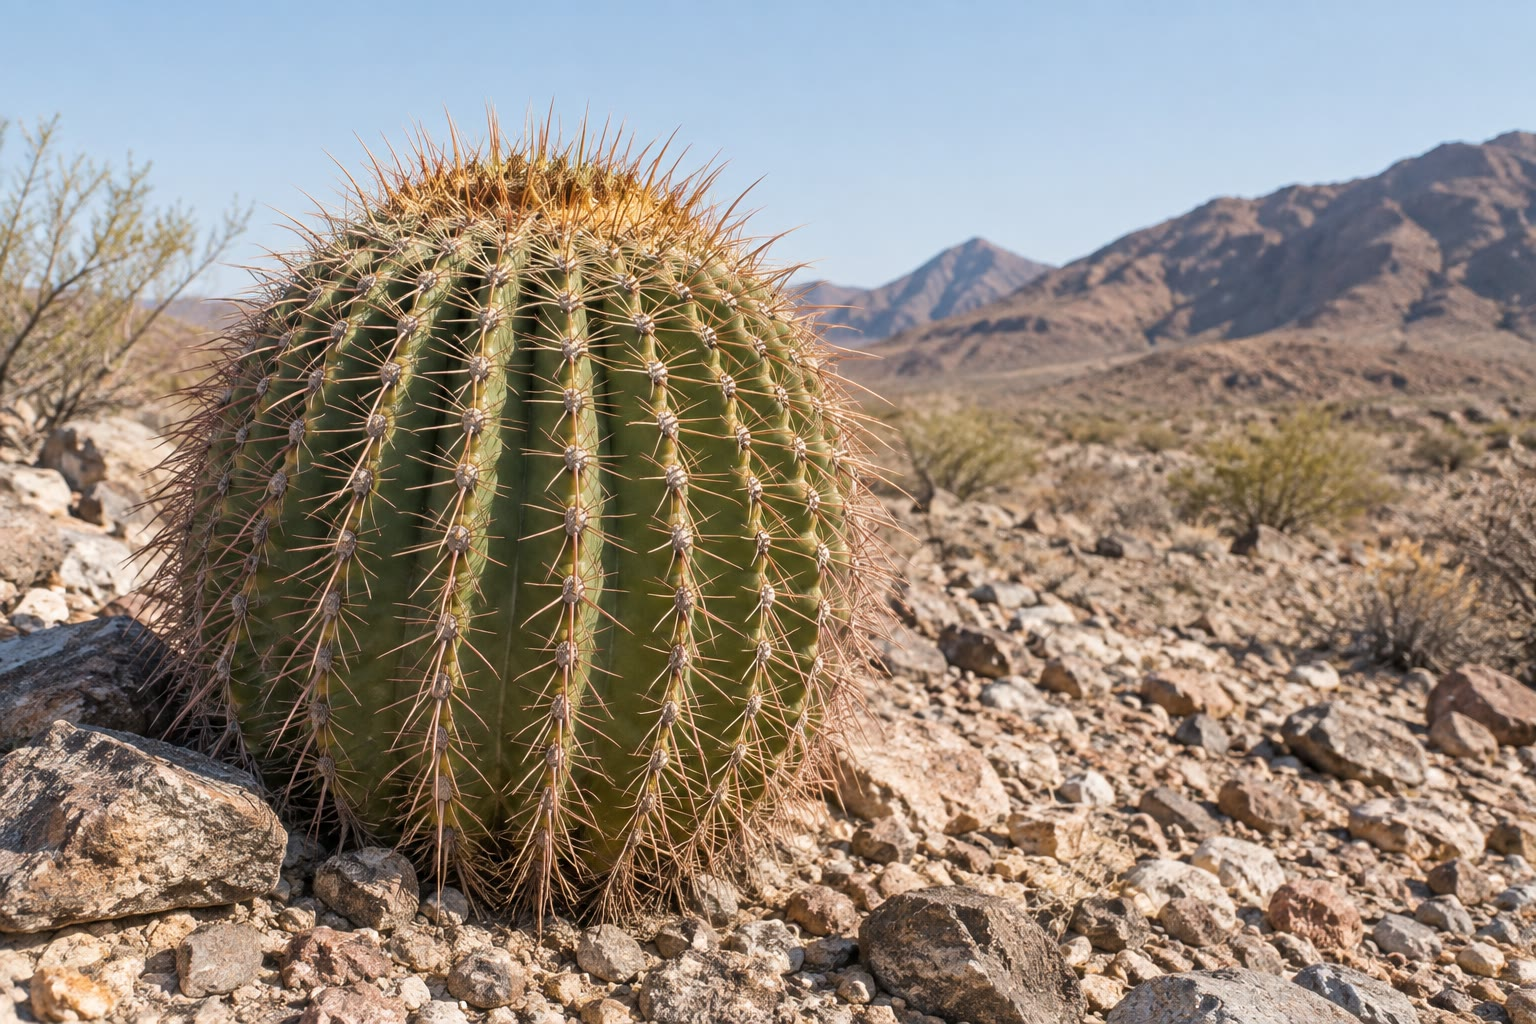
\includegraphics[width=0.55\linewidth]{images/book4/ai/b4-15-cactus.jpg}

{\small Um cacto-barril: um caule suculento com cutícula espessa,
costelas que lhe permitem inchar após a chuva, folhas reduzidas a
espinhos e estômatos que só se abrem à noite.}
\end{omfigure}

\section{Frio, sal e a resposta ao estresse}

\begin{proposition}[A aclimatação ao estresse]\label{prop:b2:plant-plasticity:stress}
\index{aclimatação ao frio}\index{halófita}\index{proteína de choque térmico}
Uma semana a \qty{4}{\celsius} baixa de \qty{-5}{\celsius} para
\qty{-25}{\celsius} a temperatura que mata um centeio de inverno: as
células acumularam açúcares e proteínas que baixam o ponto de
congelamento e protegem as membranas, mudaram seus lipídios para que
permaneçam fluidos e produziram proteínas anticongelantes que impedem
o crescimento dos cristais de gelo; o evento letal não é o gelo, que
se forma sem dano entre as células, mas a desidratação da célula à
medida que a água sai dela para se juntar ao gelo. Algumas horas a
\qty{40}{\celsius} induzem \emph{\omterm{prop:b2:plant-plasticity:stress}{proteínas de choque térmico}}, que
redobram proteínas desnaturadas e protegem a célula a
\qty{45}{\celsius}. O sal é enfrentado por exclusão na raiz,
compartimentalização no vacúolo (com solutos compatíveis no citosol
para equilibrá-lo) e, nas verdadeiras \emph{halófitas}, secreção por
glândulas de sal. A maioria dessas respostas passa pela mesma
sinalização: um sensor, uma elevação do cálcio citosólico, o \omterm{def:b2:plant-flowering:dormancy}{ácido
abscísico} e um conjunto de \omterm{prop:b2:cell-differentiation:transcriptional}{fatores de transcrição} que ativam centenas
de genes protetores --- um programa de estresse tão geral quanto a
resposta imune de um animal e, como ela, caro: a planta aclimatada
cresce devagar, e uma planta que se aclimata sem necessidade perde para
uma que não o faz.
\end{proposition}
\begin{proof}[Evidências]
Os experimentos de \omterm{prop:b2:plant-plasticity:stress}{aclimatação ao frio} medem a temperatura na qual
metade das células de uma folha morre (a LT$_{50}$) antes e depois de
um período a baixa temperatura; o deslocamento, de dez a vinte graus em
uma semana, é revertido por uma semana de calor. Mutantes incapazes de
ativar o programa do frio (os \omterm{prop:b2:cell-differentiation:transcriptional}{fatores de transcrição} CBF) se aclimatam
mal, e plantas que expressam esses fatores de forma constitutiva
sobrevivem à geada sem \omterm{def:b2:plant-plasticity:plasticity}{aclimatação} --- mas crescem como anãs.
\end{proof}

\begin{omfigure}
\begin{tikzpicture}[every node/.style={font=\scriptsize}, >=stealth]
  \node[draw, rounded corners, fill=omExo!25, align=center] (s) at (0,0) {estresse\\seca, frio,\\sal, calor};
  \node[draw, rounded corners, fill=omDef!15, align=center] (sen) at (3.2,0) {sensor\\(membrana, turgescência,\\proteínas desdobradas)};
  \node[draw, rounded corners, fill=omDef!15, align=center] (ca) at (6.4,0) {segundos mensageiros\\Ca$^{2+}$, ABA};
  \node[draw, rounded corners, fill=omProp!20, align=center] (tf) at (9.6,0) {fatores de\\transcrição};
  \node[draw, rounded corners, fill=omThm!15, align=center] (out) at (12.8,0.9) {genes protetores:\\solutos, anticongelantes,\\chaperonas, transportadores};
  \node[draw, rounded corners, fill=omThm!15, align=center] (out2) at (12.8,-0.9) {crescimento mais lento:\\o custo};
  \draw[->, thick] (s) -- (sen); \draw[->, thick] (sen) -- (ca); \draw[->, thick] (ca) -- (tf);
  \draw[->, thick] (tf) -- (out); \draw[->, thick] (tf) -- (out2);
\end{tikzpicture}

{\small A forma comum da resposta de uma planta ao estresse: um sensor,
um sinal de cálcio e de \omterm{def:b2:plant-flowering:dormancy}{ácido abscísico}, \omterm{prop:b2:cell-differentiation:transcriptional}{fatores de transcrição} e um
programa de genes protetores --- pago em crescimento.}
\end{omfigure}

\begin{example}[Sinais que mentem]\label{ex:b2:plant-plasticity:lie}
A plasticidade só é tão boa quanto o sinal. Uma plântula sob a sombra
de vermelho extremo de uma vizinha se alonga --- corretamente, se a
vizinha for uma plântula que ela possa ultrapassar; fatalmente, se for
uma árvore, pois as reservas gastas no caule se perdem para a raiz e a
folha. As culturas plantadas densamente se sombreiam, se alongam e
acamam; os melhoristas selecionaram trigos e arrozes que ignoram o
sinal de vermelho extremo. Uma semana quente em fevereiro faz brotar
folhas que uma geada de março mata; as plantas que sobrevivem são as
que também contam o frio (\cref{ch:b2:plant-flowering}). Toda resposta plástica é uma
aposta na honestidade do sinal, e a \omterm{def:b2:plant-plasticity:plasticity}{norma de reação} é moldada pela
frequência com que, no passado da linhagem, o sinal disse a verdade.
\end{example}

\section{Exercícios}

\begin{exercise}[$\star$]\label{exo:b2:plant-plasticity:1}
Defina \omterm{def:b2:plant-plasticity:plasticity}{plasticidade fenotípica}, \omterm{def:b2:plant-plasticity:plasticity}{norma de reação}, \omterm{def:b2:plant-plasticity:plasticity}{aclimatação} e
\omterm{def:b2:plant-plasticity:plasticity}{adaptação}, com um exemplo vegetal de cada uma.
\end{exercise}

\begin{exercise}[$\star$]\label{exo:b2:plant-plasticity:2}
Descreva os quatro tratamentos de Darwin com coleóptilos e o que cada um mostrou.
\end{exercise}

\begin{exercise}[$\star$]\label{exo:b2:plant-plasticity:3}
Liste cinco diferenças entre uma \omterm{prop:b2:plant-plasticity:sunshade}{folha de sol} e uma \omterm{prop:b2:plant-plasticity:sunshade}{folha de sombra}, e
diga em que momento da vida da folha a escolha é feita.
\end{exercise}

\begin{exercise}[$\star$]\label{exo:b2:plant-plasticity:4}
Como um estômato se abre, o que o abre pela manhã e o que o fecha numa
seca?
\end{exercise}

\begin{exercise}[$\star\star$]\label{exo:b2:plant-plasticity:5}
Calcule $\varphi$ para $R{:}FR = 1.15$ (sol), $0.7$ (uma clareira),
$0.2$ (sob um dossel) e $0.05$ (sombra profunda), com $a = 0.77$. Entre
quais desses valores a planta ativa a \omterm{thm:b2:plant-plasticity:phytochrome}{evitação da sombra}, se o limiar
for $\varphi = 0.4$?
\end{exercise}

\begin{exercise}[$\star\star$]\label{exo:b2:plant-plasticity:6}
Uma folha tem $g_s = \qty{0.25}{mol.m^{-2}.s^{-1}}$, $w_i - w_a = 0.025$,
$c_a - c_i = \qty{100}{\micro mol/mol}$. Calcule $E$, $A$, a eficiência
do uso da água em mols e em gramas de água por grama de carbono, e a
água perdida por metro quadrado num dia de 12 horas.
\end{exercise}

\begin{exercise}[$\star\star$]\label{exo:b2:plant-plasticity:7}
Refaça o exercício anterior para uma \omterm{prop:b2:plant-plasticity:xerophytes}{planta CAM} cujos estômatos se abrem
à noite, com $w_i - w_a = 0.005$ e a mesma condutância. Por que fator o
custo em água do carbono é reduzido?
\end{exercise}

\begin{exercise}[$\star\star$]\label{exo:b2:plant-plasticity:8}
Um estatólito é um grão de amido de raio \qty{2}{\micro m} e densidade
\qty{1500}{kg/m^3} num citoplasma de densidade \qty{1100}{kg/m^3} e
viscosidade \qty{0.01}{Pa.s}. Calcule sua velocidade de sedimentação
(Stokes) e o tempo para atravessar uma célula de \qty{10}{\micro m}.
Por que um clinostato que gira uma vez por minuto abole o
gravitropismo?
\end{exercise}

\begin{exercise}[$\star\star$]\label{exo:b2:plant-plasticity:9}
Um caule de \qty{2}{mm} de diâmetro cresce \qty{2}{\%} por hora numa
zona de \qty{20}{mm}. A luz vinda de um lado reparte a auxina em
$60 : 40$. Em que ângulo ele se curvou após duas horas? Após quanto
tempo ele fica a \qty{90}{\degree} de sua direção original?
\end{exercise}

\begin{exercise}[$\star\star\star$]\label{exo:b2:plant-plasticity:10}
Uma plântula com \qty{50}{mg} de reservas se alonga \qty{2}{cm} por dia
em campo aberto e \qty{4}{cm} por dia sob um dossel, gastando
\qty{1}{mg} de reservas por centímetro de caule além do que suas folhas
fornecem. O dossel está \qty{30}{cm} acima dela num urtigal e
\qty{10}{m} acima num bosque. Em que caso a \omterm{thm:b2:plant-plasticity:phytochrome}{evitação da sombra} dá
certo, e o que acontece no outro?
\end{exercise}

\begin{exercise}[$\star\star\star$]\label{exo:b2:plant-plasticity:11}
Explique por que o congelamento mata uma célula por desidratação, e não
pelo gelo, o que uma semana de frio faz para impedi-lo, e por que uma
planta que expressa o programa do frio o ano todo é anã.
\end{exercise}

\begin{exercise}[$\star\star\star$]\label{exo:b2:plant-plasticity:12}
``A plasticidade é uma aposta na honestidade de um sinal.'' Discuta com
o sinal de vermelho extremo, a semana quente de fevereiro e o
melhoramento de culturas que ignoram suas vizinhas.
\end{exercise}

\section{Problema: Uma plântula sob o dossel}

\begin{problem}[{Problema de fim de semana --- o clima luminoso, o
alongamento, o balanço hídrico e os tropismos de uma plântula
calculados a partir da física de seus sensores, até o estado de seu
fitocromo, sua altura após uma quinzena e seu uso diário de água}]
\label{pb:b2:plant-plasticity:1}
Uma plântula de bétula germina sob um dossel que transmite \qty{3}{\%}
da luz do sol e reduz $R{:}FR$ de $1.15$ para $0.2$ ($a = 0.77$). Em
sol pleno, ela se alongaria a \qty{1.5}{cm} por dia; sob o dossel, sua
taxa de alongamento é multiplicada por $1 +
2(0.6 - \varphi)$. Seu caule tem \qty{2}{mm} de diâmetro, com uma zona
de crescimento de \qty{15}{mm}. Folhas: \qty{20}{cm^2} no total;
$g_s =
\qty{0.2}{mol.m^{-2}.s^{-1}}$; $w_i - w_a = 0.015$ na sombra, $0.03$
numa clareira; $c_a - c_i = \qty{80}{\micro mol/mol}$; o dia dura
\qty{14}{h}. Estatólitos: raio de \qty{2.5}{\micro m}, densidade de
\qty{1500}{kg/m^3}, num citoplasma de \qty{1100}{kg/m^3} e
\qty{0.01}{Pa.s}.

\medskip
\noindent\textbf{Parte I --- A luz.}
\begin{enumerate}
  \item Calcule $\varphi$ em campo aberto e sob o dossel.
  \item O que a plântula conclui a partir de $\varphi$, e o que
        concluiria se o dossel transmitisse \qty{3}{\%} da luz sem mudar
        sua cor (uma tela de sombreamento)?
  \item Calcule a taxa de alongamento sob o dossel.
  \item Qual é a altura da plântula após 14 dias ali, em comparação com
        uma irmã em campo aberto?
  \item Abre-se uma clareira de um lado, elevando $R{:}FR$ desse lado
        para $0.8$. Que duas respostas se seguem, e por quais dois
        fotorreceptores?
  \item Por que as folhas desenvolvidas sob o dossel são maiores e mais
        finas, e o que acontece com elas se o dossel for derrubado?
\end{enumerate}

\medskip
\noindent\textbf{Parte II --- A curvatura em direção à clareira.}
\begin{enumerate}[resume]
  \item A luz da clareira reparte a auxina em $65 : 35$ através do
        caule. Com a taxa de alongamento sob o dossel da questão 3,
        calcule a extensão relativa de cada lado da zona de crescimento
        em uma hora.
  \item Calcule o ângulo de curvatura após uma hora.
  \item Após quanto tempo o caule aponta diretamente para a clareira, se
        a clareira está a \qty{60}{\degree} da vertical?
  \item O caule agora está inclinado. Calcule a velocidade de
        sedimentação de um estatólito e o tempo para atravessar uma
        célula de \qty{12}{\micro m}.
  \item O gravitropismo e o fototropismo do caule agora discordam. Qual
        vence numa planta que evita a sombra, e por que isso é
        adaptativo?
  \item Uma raiz da mesma plântula é inclinada \qty{45}{\degree} por uma
        pedra. Preveja sua resposta e explique por que ela é oposta à do
        caule, embora o mecanismo seja o mesmo.
\end{enumerate}

\medskip
\noindent\textbf{Parte III --- A água.}
\begin{enumerate}[resume]
  \item Calcule a taxa de transpiração por metro quadrado na sombra e a
        água perdida pelas folhas da plântula num dia.
  \item Calcule o carbono fixado por metro quadrado por segundo e por
        dia, e a eficiência do uso da água em gramas de água por grama de
        carbono.
  \item Qual é o ganho diário total de carbono da plântula na sombra, em
        miligramas?
  \item Recalcule a água perdida e a eficiência na clareira.
  \item O solo seca e o \omterm{def:b2:plant-flowering:dormancy}{ácido abscísico} reduz $g_s$ a
        \qty{0.02}{mol.m^{-2}.s^{-1}}. Recalcule $E$ e $A$ (suponha que
        $c_a - c_i$ sobe para \qty{200}{\micro mol/mol}). Qual cai mais,
        e por quê?
  \item A plântula tem \qty{5}{g} de tecido foliar com \qty{85}{\%} de
        água e pode perder um quinto dessa água antes de murchar. Quanto
        tempo ela resiste na clareira, com os estômatos abertos, se as
        raízes não fornecerem nada?
  \item Explique por que uma estratégia CAM não serviria a uma plântula
        de bétula sob um dossel.
\end{enumerate}

\medskip
\noindent\textbf{Parte IV --- A aposta.}
\begin{enumerate}[resume]
  \item A plântula tem \qty{100}{mg} de reservas e gasta \qty{2}{mg}
        por centímetro de caule além do que suas folhas fornecem na
        sombra. Quanto caule ela consegue construir só com as reservas?
  \item O dossel é um urtigal \qty{40}{cm} acima; depois, um bosque
        \qty{8}{m} acima. Diga, em cada caso, se o alongamento alcança a
        luz antes que as reservas se esgotem, e qual teria sido a melhor
        resposta no bosque.
  \item A bétula é uma pioneira de terrenos abertos; uma plântula de faia
        consegue esperar décadas na sombra profunda. Compare as \omterm{def:b2:plant-plasticity:plasticity}{normas de
        reação} a $\varphi$ que se espera de cada uma.
  \item Um melhorista quer uma cultura plantada densamente que não se
        alongue. Que sensor ou resposta você desativaria, e que efeito
        colateral seria preciso verificar?
  \item Explique em duas frases por que uma planta que não percebe suas
        vizinhas e uma planta que sempre acredita nelas estão ambas em
        pior situação do que uma que às vezes acredita.
  \item Enuncie o resultado: $\varphi$ ao sol e na sombra, a altura da
        plântula após 14 dias e seu uso diário de água na sombra e na
        clareira.
\end{enumerate}
\end{problem}
